
This part of the chapter describes how the quench velocity method is applied in ANSYS simulations via Python script. In order to distinguish the quenched zone from the non-quenched one, the superconducting cable is divided into two domains as presented in Fig. \ref{fig:ansys_material_assignment}. The non-quenched part is characterised by nearly zero-resistivity for the sake of numerical stability whereas the quenched cable has nonlinear resistivity properties of copper. The material properties are reassigned at each time step as the quench propagates in ANSYS model.

\begin{figure}[H]
\centering
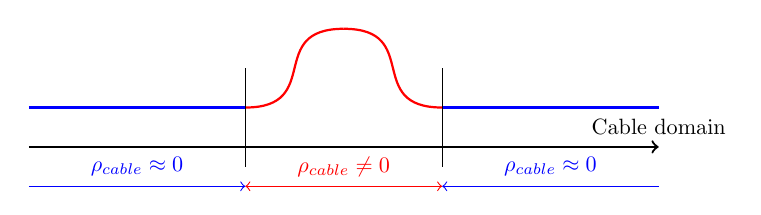
\begin{tikzpicture}[scale = 1]
\draw [thick, ->] (0.0,0.0) -- (8.0,0);
\draw [thick, blue] (0.0,0.5) -- (2.75,0.5);
\draw [thick, blue] (5.25,0.5) -- (8.0,0.5);
\draw [thick, red] (2.75,0.5) .. controls +(0:1cm) and +(180:1cm) .. (4.0,1.5);
\draw [thick, red] (4.0,1.5) .. controls +(0:1cm) and +(180:1cm) .. (5.25,0.5);
\draw [thin] (2.75,-0.25) -- (2.75,1.0);
\draw [thin] (5.25,-0.25) -- (5.25,1.0);
\draw [thin, red, <->] (2.75,-0.5) -- (5.25,-0.5);
\draw [thin, blue, ->] (0.0,-0.5) -- (2.75,-0.5);
\draw [thin, blue, <-] (5.25,-0.5) -- (8.0,-0.5);
\node[scale = 0.8] [color = red] at (4.0,-0.25) {$\rho_\text{cable} \neq 0$};
\node[scale = 0.8] [color = blue] at (1.375,-0.25) {$\rho_\text{cable} \approx 0$};
\node[scale = 0.8] [color = blue] at (6.625,-0.25) {$\rho_\text{cable} \approx 0$};
\node[scale = 0.8] at (8.0,+0.25) {Cable domain};
\end{tikzpicture}
\caption{ANSYS cable domain assignment.}
    \label{fig:ansys_material_assignment}
\end{figure}

As described at the beginning of the chapter, the quench velocity can be: $(a)$ assumed constant, $(b)$ based on available measurements, $(c)$ calculated numerically, $(d)$ calculated analytically according to quench velocity equations available in literature. The first 3 above-mentioned methods to calculate quench velocity would require one-directional exchange of signals between Python and ANSYS, as described in \ref{fig:unidirectional_coupling_scheme}. The initial quench length should be assumed in Python when starting the quench velocity algorithm. Then, ANSYS environment is provided with a Python quench front position from the previous communication point $T_{j-1}$ and calculates temperature distribution in the current communication point $T_j$.

If quench velocity is analysed by means of analytic formula (like in the \nth{4} case), quench velocity algorithm should be a bidirectional exchange of signals in form of weak coupling, as presented in Fig. \ref{fig:bidirectional_coupling_scheme}. In such a case, Python script is provided with the data from ANSYS at point $T_j$ to estimate quench velocity at point $T_{j-1}$ up to the point $T_j$. The line which describes the information direction is marked in red in Fig. \ref{fig:bidirectional_coupling_scheme}.

Between the Python time steps, ANSYS solves the problem with an automatic time step where the minimum and the maximum time step is defined by a user. For the purpose of this thesis, the Python script was developed to calculate quench velocity assuming that it constant or it is calculated numerically (case a and c). The creation of a numerical map for the quench velocity will be further described in chapter \ref{section:skew_quadrupole_quench_detection_analysis}. This method is used for quench velocity modelling of a skew quadrupole.

\begin{figure}[H]
\centering
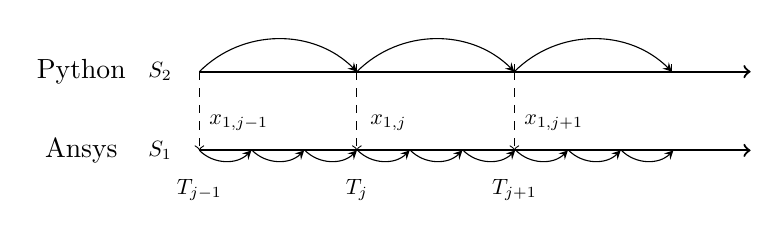
\begin{tikzpicture}[scale = 1]
\draw[thick,->] (0,1) -- (7,1);
\draw (2, 1) -- (2, 1.1);
\draw (4, 1) -- (4, 1.1);
\draw (6, 1) -- (6, 1.1);
\foreach \t in {1,3,5}
\draw [-stealth, bend angle=45, bend left, color = black]  ({\t-1},1) to (\t+1,1);
\draw[thick,->] (0,0) -- (7,0);
\draw (2, 1) -- (2, 1.1);
\draw (4, 1) -- (4, 1.1);
\draw (6, 1) -- (6, 1.1);
\foreach \t in {0.66,1.33,...,6.33}
\draw [-stealth, bend angle=45, bend right]  ({\t-0.66},0) to (\t,0);
\node[scale = 0.8] at (0, -0.5) {$T_{j-1}$};
\node[scale = 0.8] at (2,-0.5) {$T_j$};
\node[scale = 0.8] at (4,-0.5) {$T_{j+1}$};
\draw[dashed, ->] (0,1) -- (0,0);
\draw[dashed, ->] (2,1) -- (2,0);
\draw[dashed, ->] (4,1) -- (4,0);
\node[scale = 0.8] at (-0.5, 0) {$\text{S}_1$};
\node[scale = 0.8] at (-0.5, 1) {$\text{S}_2$};
\node[scale = 0.8] at (0.5, 0.35) {$\text{x}_{1,j-1}$};
\node[scale = 0.8] at (2.4, 0.35) {$\text{x}_{1,j}$};
\node[scale = 0.8] at (4.5, 0.35) {$\text{x}_{1,j+1}$};
\node[color = black] at (-1.5,1.0)	{Python};
\node at (-1.5,0)	{Ansys};
\end{tikzpicture}
\caption{Schematic representation of unidirectional coupling between ANSYS and external Python code.}
\label{fig:unidirectional_coupling_scheme}
\end{figure}

\begin{figure}[H]
\centering
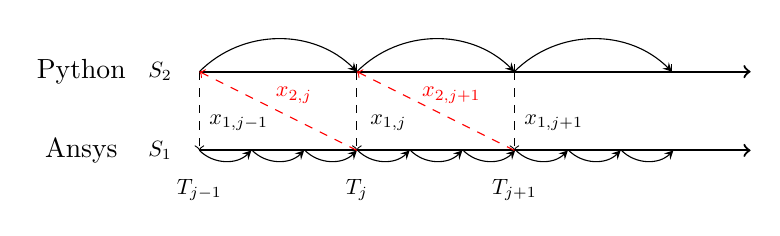
\begin{tikzpicture}[scale = 1]
\draw[thick,->] (0,1) -- (7,1);
\draw (2, 1) -- (2, 1.1);
\draw (4, 1) -- (4, 1.1);
\draw (6, 1) -- (6, 1.1);
\foreach \t in {1,3,5}
\draw [-stealth, bend angle=45, bend left, color = black]  ({\t-1},1) to (\t+1,1);
\draw[thick,->] (0,0) -- (7,0);
\draw (2, 1) -- (2, 1.1);
\draw (4, 1) -- (4, 1.1);
\draw (6, 1) -- (6, 1.1);
\foreach \t in {0.66,1.33,...,6.33}
\draw [-stealth, bend angle=45, bend right]  ({\t-0.66},0) to (\t,0);
\node[scale = 0.8] at (0, -0.5) {$T_{j-1}$};
\node[scale = 0.8] at (2,-0.5) {$T_j$};
\node[scale = 0.8] at (4,-0.5) {$T_{j+1}$};
\draw[dashed, ->] (0,1) -- (0,0);
\draw[dashed, ->] (2,1) -- (2,0);
\draw[dashed, ->] (4,1) -- (4,0);
\draw[dashed, red, ->] (2,0) -- (0,1);
\draw[dashed, red, ->] (4,0) -- (2,1);
\node[scale = 0.8] at (-0.5, 0) {$\text{S}_1$};
\node[scale = 0.8] at (-0.5, 1) {$\text{S}_2$};
\node[scale = 0.8] at (0.5, 0.35) {$\text{x}_{1,j-1}$};
\node[scale = 0.8] at (2.4, 0.35) {$\text{x}_{1,j}$};
\node[scale = 0.8] at (4.5, 0.35) {$\text{x}_{1,j+1}$};
\node[scale = 0.8, red] at (1.2, 0.7) {$\text{x}_{2,j}$};
\node[scale = 0.8, red] at (3.2, 0.7) {$\text{x}_{2,j+1}$};
\node[color = black] at (-1.5,1.0)	{Python};
\node at (-1.5,0)	{Ansys};
\end{tikzpicture}
\caption{Schematic representation of bidirectional coupling between ANSYS and external Python code.}
\label{fig:bidirectional_coupling_scheme}
\end{figure}

Provided that data exchange between Python module and ANSYS occurs at communication times $T_j$, the quench velocity algorithm is solved as described in Algorithm \ref{alg:weak_coupling}.

\begin{algorithm}
  \caption{Weak Coupling between ANSYS and Python environment}
  \label{alg:weak_coupling}
  \begin{algorithmic}[1]
    \STATE assume initial quench position $x_{1,j-1}$ 
    \STATE \textbf{for} $j=1,2,...,N$ \textbf{do}
    \STATE \hspace{0.5cm} solve temperature distribution at time $T_j$
    \STATE \hspace{0.5cm} extrapolate ANSYS results $x_{2,j}$ to Python step $T_{j-1}$ (bidirectional case from Fig. \ref{fig:bidirectional_coupling_scheme})
    \STATE \hspace{0.5cm} estimate new quench position $x_{1,j}$ for each existing quench front
    \STATE \hspace{0.5cm} assign quench position $x_{1,j}$ to new nodes for ANSYS time step $T_j$
  \end{algorithmic}
\end{algorithm}
